\subsection{Reading Schematics}
\label{subsec:schem-reading}

When you first look at a schematic diagram, it might seem like a jumble of lines and symbols. But don't worry, it's not as complicated as it looks! A schematic is essentially a map of an electrical circuit, showing how components are connected together. It uses standardized symbols to represent different components, making it easier for engineers and hobbyists to understand and build circuits without needing to know what each component looks like physically.

\subsubsection*{The Purpose of Schematics}
The primary purpose of a schematic is to provide a clear and concise representation of an electrical circuit. Unlike a physical layout, which shows where components are placed on a board, a schematic focuses on the connections between components. This allows you to understand how the circuit functions without getting bogged down by the physical arrangement.

\subsubsection*{Standard Symbols in Schematics}
In schematics, each component is represented by a unique symbol. For example, a resistor is typically shown as a zigzag line, while a transistor might be represented by a combination of lines and arrows. Batteries are often depicted as a series of long and short lines, and the ground symbol is usually a horizontal line with three downward-pointing lines. These symbols are standardized, so once you learn them, you can read any schematic.

\subsubsection*{Identifying Components}
Let's take a closer look at some common components and their symbols:

\begin{itemize}
    \item \textbf{Resistor}: Represented by a zigzag line. Resistors are used to limit the flow of current in a circuit.
    \item \textbf{Transistor}: Typically shown as a combination of lines and arrows. Transistors are used to amplify or switch electronic signals.
    \item \textbf{Battery}: Depicted as a series of long and short lines. Batteries provide the power needed to run the circuit.
    \item \textbf{Ground Symbol}: A horizontal line with three downward-pointing lines. This symbol represents the reference point in a circuit, often connected to the earth or a common return path.
\end{itemize}

\subsubsection*{Capacitors and Inductors}
Capacitors and inductors are also common in electronic circuits. Capacitors, represented by two parallel lines, store electrical energy, while inductors, shown as a series of loops, store energy in a magnetic field. Both components are crucial for filtering and tuning circuits.

\subsubsection*{Light-Emitting Diodes (LEDs)}
LEDs are represented by a triangle with a line pointing away from it, often with a small arrow indicating the direction of light emission. LEDs are used to indicate the status of a circuit or to provide illumination.

\subsubsection*{Variable Components}
Variable components, like resistors and inductors, are represented with an arrow through their standard symbols. These components allow you to adjust the resistance or inductance in a circuit, making them useful for tuning and calibration.

\subsubsection*{Transformers}
Transformers are depicted as two coils with a line between them. They are used to step up or step down voltage levels in a circuit, making them essential for power supply designs.

\subsubsection*{Antennas}
Antennas are represented by a simple line with a small triangle at the end. They are used to transmit or receive radio signals, making them a key component in radio circuits.

\begin{figure}[h]
    \centering
    %\includegraphics[width=0.8\textwidth]{schematic-example}
    \caption{Example schematic diagram with standard electronic components.}
    \label{fig:schematic-example}
    % Prompt: A detailed schematic diagram showing common electronic components like resistors, capacitors, transistors, and LEDs.
\end{figure}

\begin{figure}[h]
    \centering
    %\includegraphics[width=0.8\textwidth]{component-symbols}
    \caption{Comparison of physical components and their schematic symbols.}
    \label{fig:component-symbols}
    % Prompt: A comparison of physical components and their schematic symbols.
\end{figure}

\begin{table}[h]
    \centering
    \begin{tabular}{|c|c|}
        \hline
        \textbf{Component} & \textbf{Schematic Symbol} \\
        \hline
        Resistor & Zigzag line \\
        Transistor & Lines and arrows \\
        Battery & Long and short lines \\
        Ground & Horizontal line with three downward lines \\
        Capacitor & Two parallel lines \\
        Inductor & Series of loops \\
        LED & Triangle with a line and arrow \\
        Variable Resistor & Zigzag line with an arrow \\
        Transformer & Two coils with a line \\
        Antenna & Line with a triangle \\
        \hline
    \end{tabular}
    \caption{Common electronic components and their schematic symbols.}
    \label{tab:component-symbols}
\end{table}

\subsubsection*{Questions}

\begin{tcolorbox}[colback=gray!10!white,colframe=black!75!black,title={T6C01}]
    What is the name of an electrical wiring diagram that uses standard component symbols?
    \begin{enumerate}[label=\Alph*),noitemsep]
        \item Bill of materials
        \item Connector pinout
        \item \textbf{Schematic}
        \item Flow chart
    \end{enumerate}
\end{tcolorbox}
A schematic is the correct term for an electrical wiring diagram that uses standard component symbols. The other options refer to different types of documentation.



\begin{tcolorbox}[
    colback=gray!10!white,
    colframe=black!75!black,
    title={T6C02},
    sidebyside,
    sidebyside align=top,
    lefthand width=0.45\textwidth
]
What is component 1 in figure T-1?
\begin{enumerate}[label=\Alph*),noitemsep]
    \item \textbf{Resistor}
    \item Transistor
    \item Battery
    \item Connector
\end{enumerate}
\tcblower
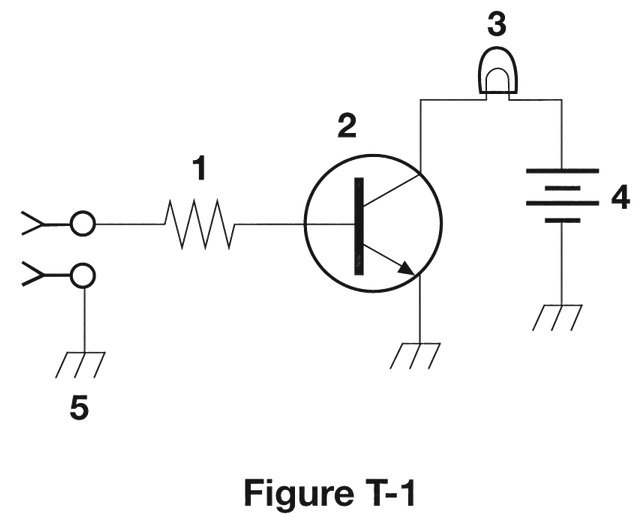
\includegraphics[width=0.7\textwidth]{tech/images/t1.png}
\end{tcolorbox}
Component 1 in figure T-1 is a resistor. Resistors are commonly represented by a zigzag line in schematics.

\begin{tcolorbox}[
    colback=gray!10!white,
    colframe=black!75!black,
    title={T6C03},
    sidebyside,
    sidebyside align=top,
    lefthand width=0.45\textwidth
]
What is component 2 in figure T-1?
\begin{enumerate}[label=\Alph*),noitemsep]
    \item Resistor
    \item \textbf{Transistor}
    \item Indicator lamp
    \item Connector
\end{enumerate}
\tcblower
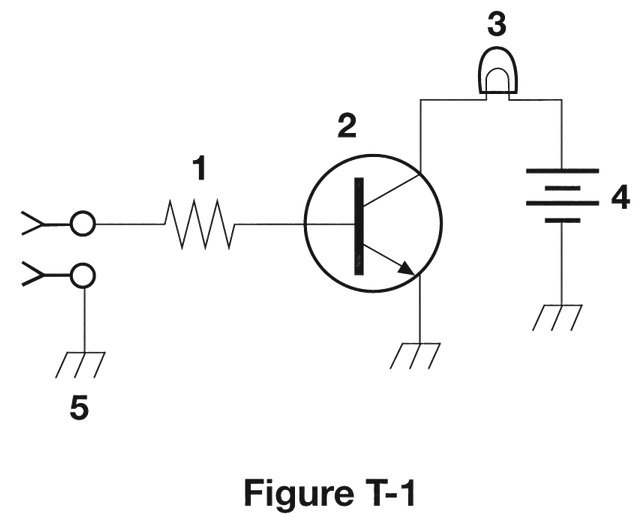
\includegraphics[width=0.7\textwidth]{tech/images/t1.png}
\end{tcolorbox}
Component 2 in figure T-1 is a transistor. Transistors are typically represented by a combination of lines and arrows.

\begin{tcolorbox}[
    colback=gray!10!white,
    colframe=black!75!black,
    title={T6C04},
    sidebyside,
    sidebyside align=top,
    lefthand width=0.45\textwidth
]
What is component 3 in figure T-1?
\begin{enumerate}[label=\Alph*),noitemsep]
    \item Resistor
    \item Transistor
    \item \textbf{Lamp}
    \item Ground symbol
\end{enumerate}
\tcblower
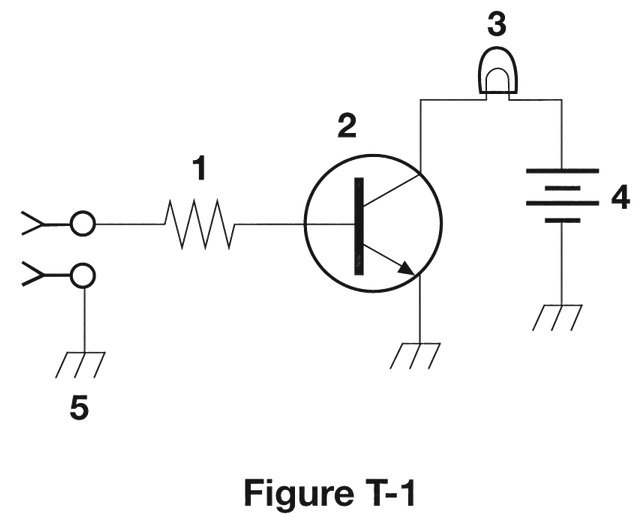
\includegraphics[width=0.7\textwidth]{tech/images/t1.png}
\end{tcolorbox}
Component 3 in figure T-1 is a lamp. Lamps are often represented by a circle with a cross inside.

\begin{tcolorbox}[
    colback=gray!10!white,
    colframe=black!75!black,
    title={T6C05},
    sidebyside,
    sidebyside align=top,
    lefthand width=0.45\textwidth
]
What is component 4 in figure T-1?
\begin{enumerate}[label=\Alph*),noitemsep]
    \item Resistor
    \item Transistor
    \item Ground symbol
    \item \textbf{Battery}
\end{enumerate}
\tcblower
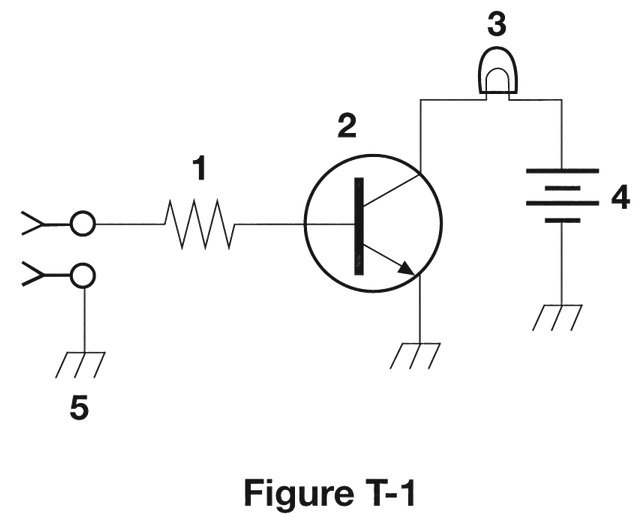
\includegraphics[width=0.7\textwidth]{tech/images/t1.png}
\end{tcolorbox}
Component 4 in figure T-1 is a battery. Batteries are typically represented by a series of long and short lines.



\begin{tcolorbox}[
    colback=gray!10!white,
    colframe=black!75!black,
    title={T6C06},
    sidebyside,
    sidebyside align=top,
    lefthand width=0.45\textwidth
]
What is component 6 in figure T-2?
\begin{enumerate}[label=\Alph*),noitemsep]
    \item Resistor
    \item \textbf{Capacitor}
    \item Regulator IC
    \item Transistor
\end{enumerate}
\tcblower
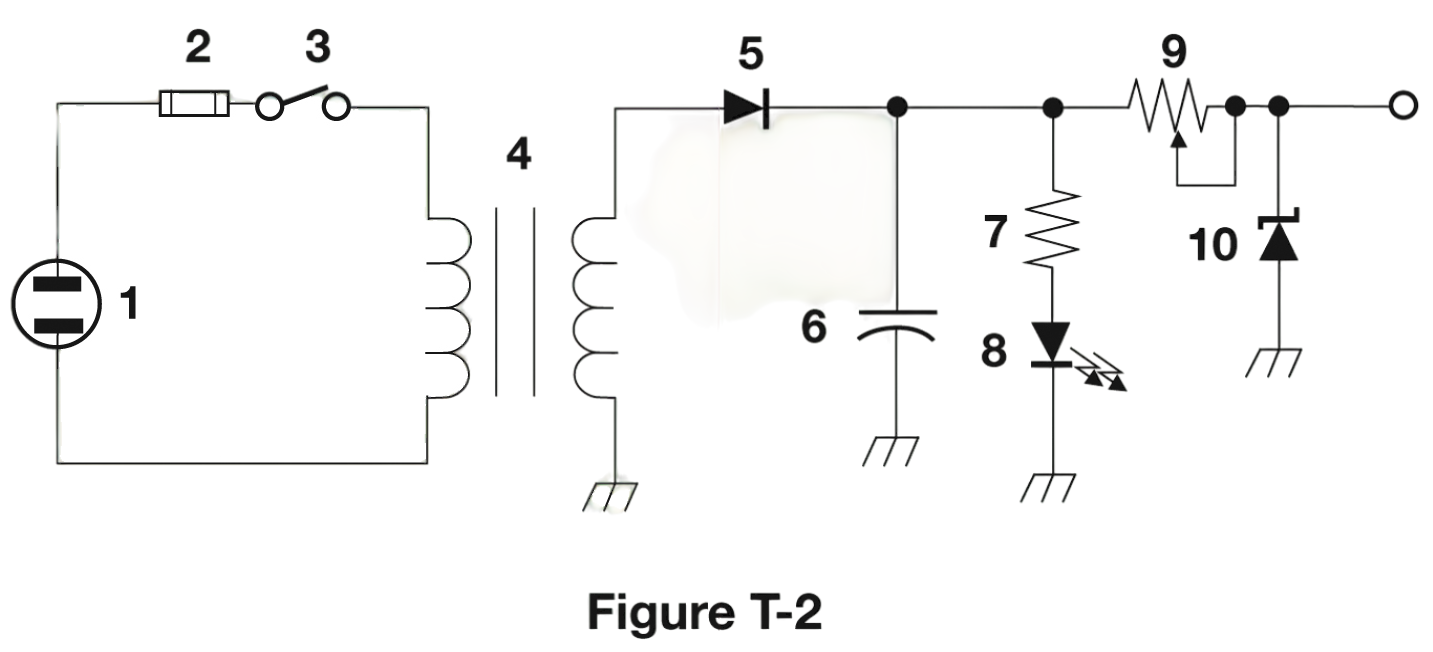
\includegraphics[width=0.7\textwidth]{tech/images/t2.png}
\end{tcolorbox}
Component 6 in figure T-2 is a capacitor. Capacitors are represented by two parallel lines in schematics.

\begin{tcolorbox}[
    colback=gray!10!white,
    colframe=black!75!black,
    title={T6C07},
    sidebyside,
    sidebyside align=top,
    lefthand width=0.45\textwidth
]
What is component 8 in figure T-2?
\begin{enumerate}[label=\Alph*),noitemsep]
    \item Resistor
    \item Inductor
    \item Regulator IC
    \item \textbf{Light emitting diode}
\end{enumerate}
\tcblower
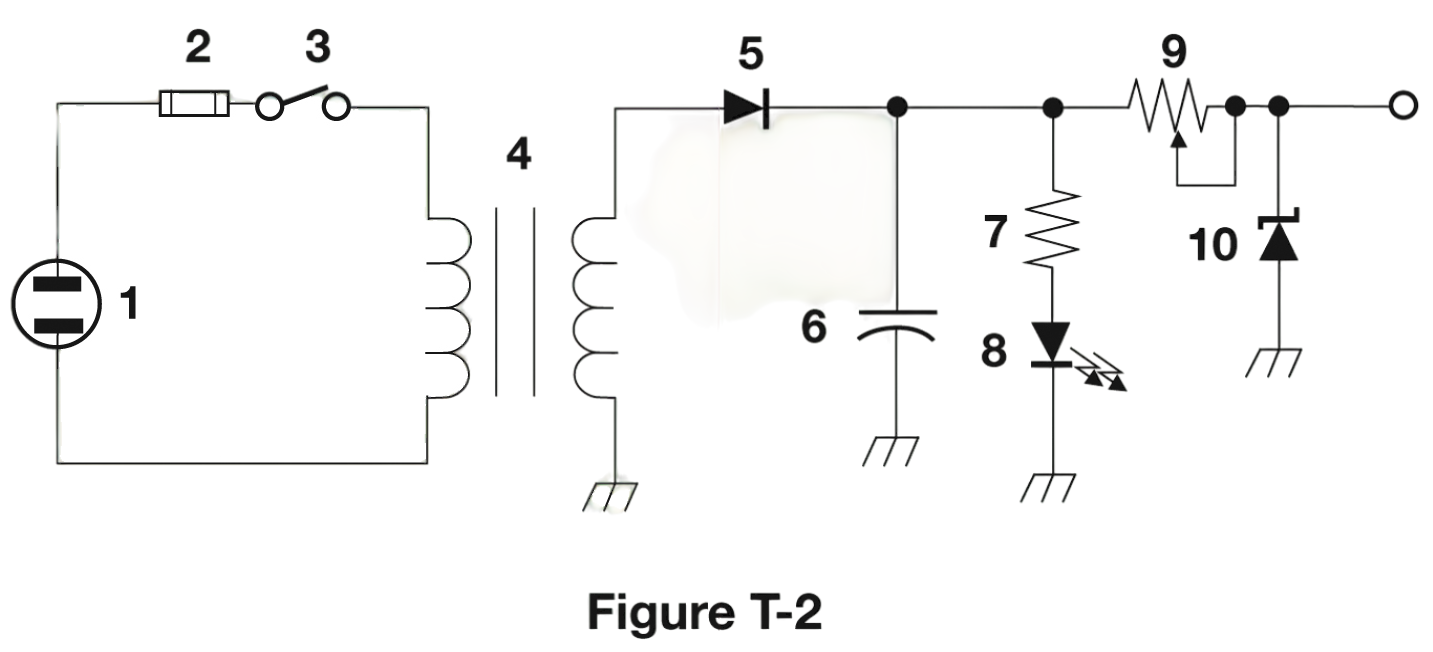
\includegraphics[width=0.7\textwidth]{tech/images/t2.png}
\end{tcolorbox}
Component 8 in figure T-2 is a light-emitting diode (LED). LEDs are represented by a triangle with a line and arrow.

\begin{tcolorbox}[
    colback=gray!10!white,
    colframe=black!75!black,
    title={T6C08},
    sidebyside,
    sidebyside align=top,
    lefthand width=0.45\textwidth
]
What is component 9 in figure T-2?
\begin{enumerate}[label=\Alph*),noitemsep]
    \item Variable capacitor
    \item Variable inductor
    \item \textbf{Variable resistor}
    \item Variable transformer
\end{enumerate}
\tcblower
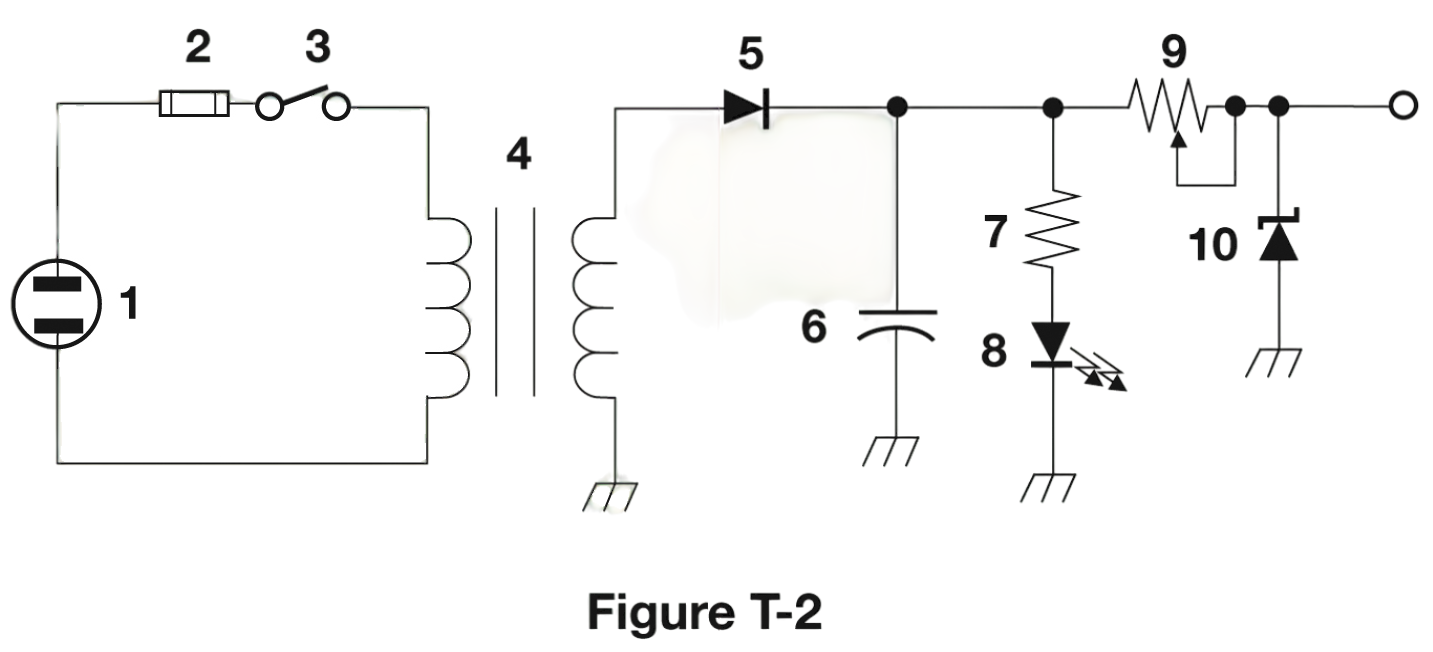
\includegraphics[width=0.7\textwidth]{tech/images/t2.png}
\end{tcolorbox}
Component 9 in figure T-2 is a variable resistor. Variable resistors are represented by a zigzag line with an arrow.

\begin{tcolorbox}[
    colback=gray!10!white,
    colframe=black!75!black,
    title={T6C09},
    sidebyside,
    sidebyside align=top,
    lefthand width=0.45\textwidth
]
What is component 4 in figure T-2?
\begin{enumerate}[label=\Alph*),noitemsep]
    \item Variable inductor
    \item Double-pole switch
    \item Potentiometer
    \item \textbf{Transformer}
\end{enumerate}
\tcblower
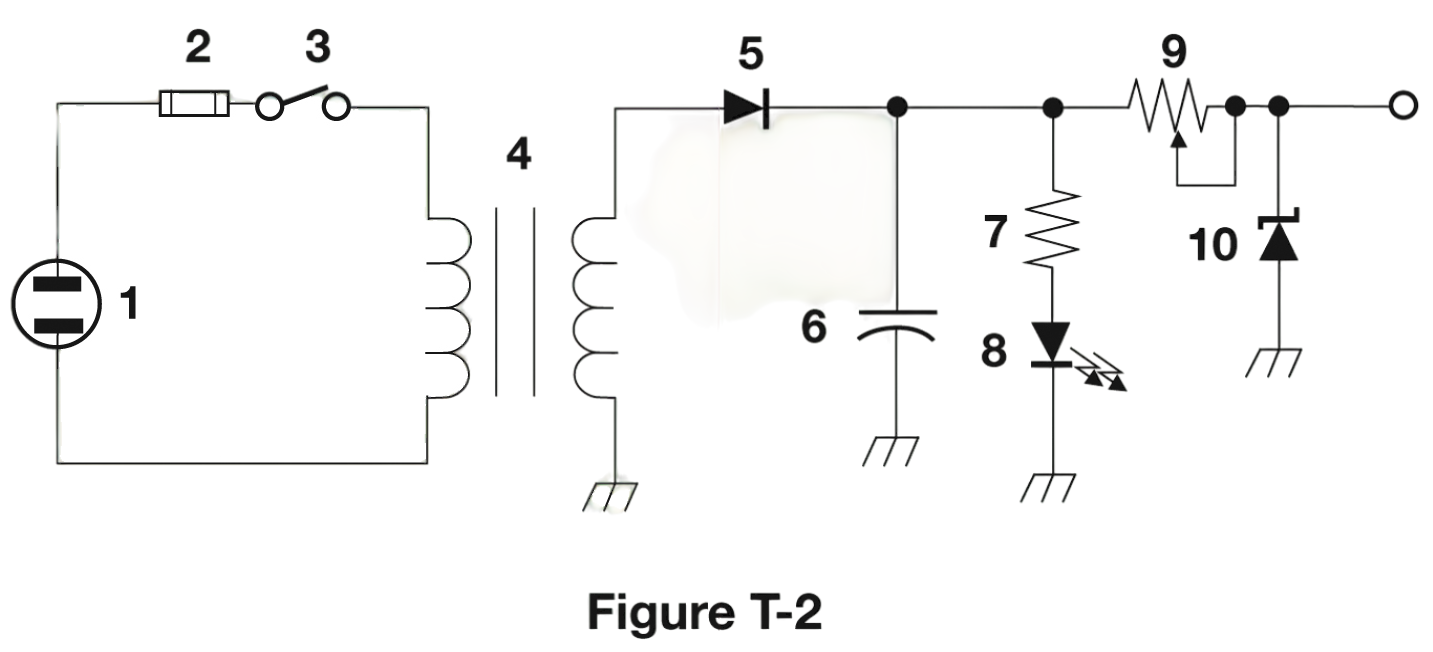
\includegraphics[width=0.7\textwidth]{tech/images/t2.png}
\end{tcolorbox}
Component 4 in figure T-2 is a transformer. Transformers are represented by two coils with a line between them.

\begin{tcolorbox}[
    colback=gray!10!white,
    colframe=black!75!black,
    title={T6C10},
    sidebyside,
    sidebyside align=top,
    lefthand width=0.45\textwidth
]
What is component 3 in figure T-3?
\begin{enumerate}[label=\Alph*),noitemsep]
    \item Connector
    \item Meter
    \item Variable capacitor
    \item \textbf{Variable inductor}
\end{enumerate}
\tcblower
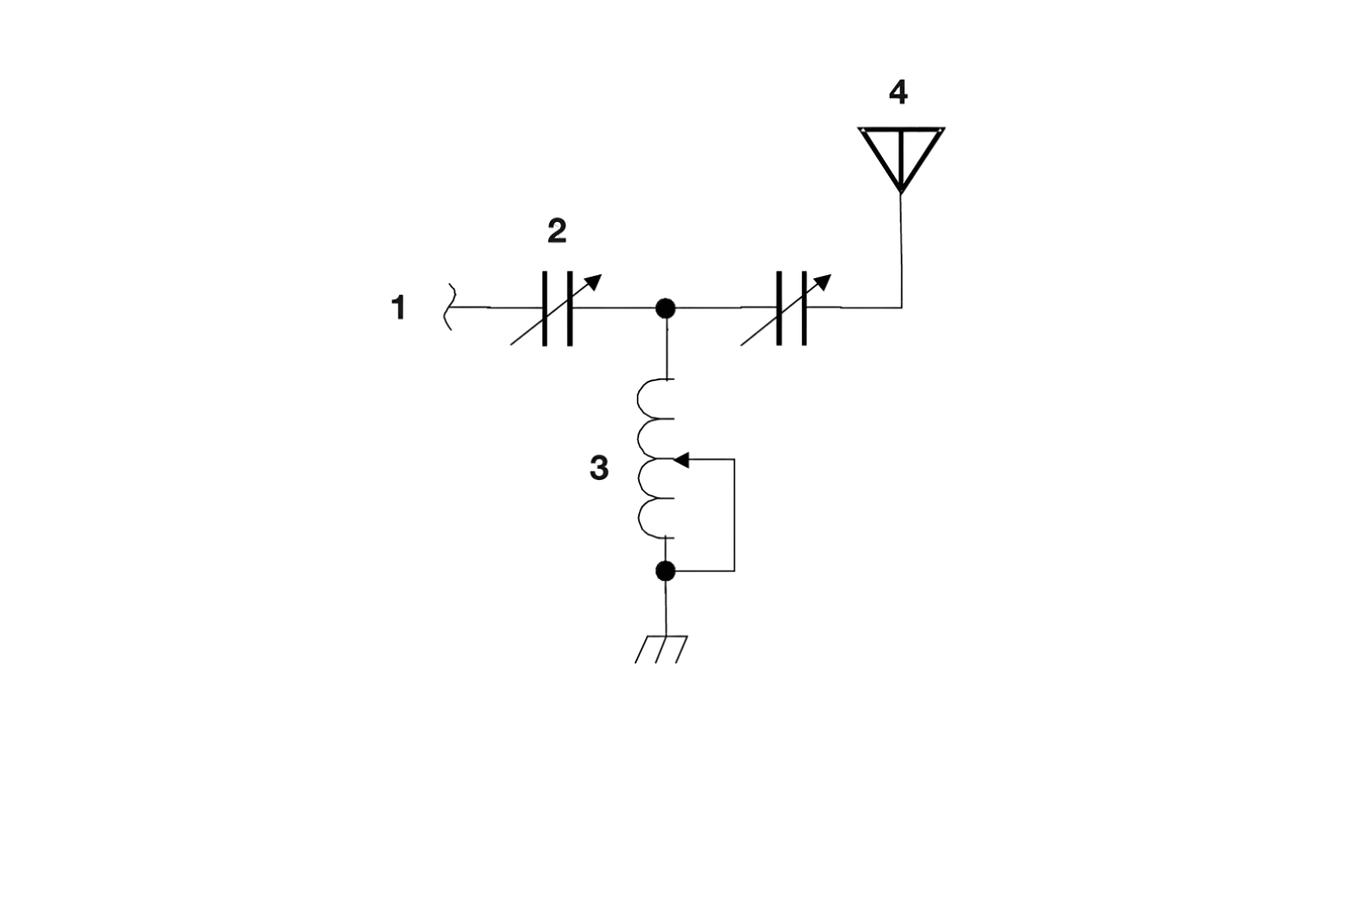
\includegraphics[width=0.7\textwidth]{tech/images/t3.png}
\end{tcolorbox}
Component 3 in figure T-3 is a variable inductor. Variable inductors are represented by a series of loops with an arrow.

\begin{tcolorbox}[
    colback=gray!10!white,
    colframe=black!75!black,
    title={T6C11},
    sidebyside,
    sidebyside align=top,
    lefthand width=0.45\textwidth
]
What is component 4 in figure T-3?
\begin{enumerate}[label=\Alph*),noitemsep]
    \item \textbf{Antenna}
    \item Transmitter
    \item Dummy load
    \item Ground
\end{enumerate}
\tcblower
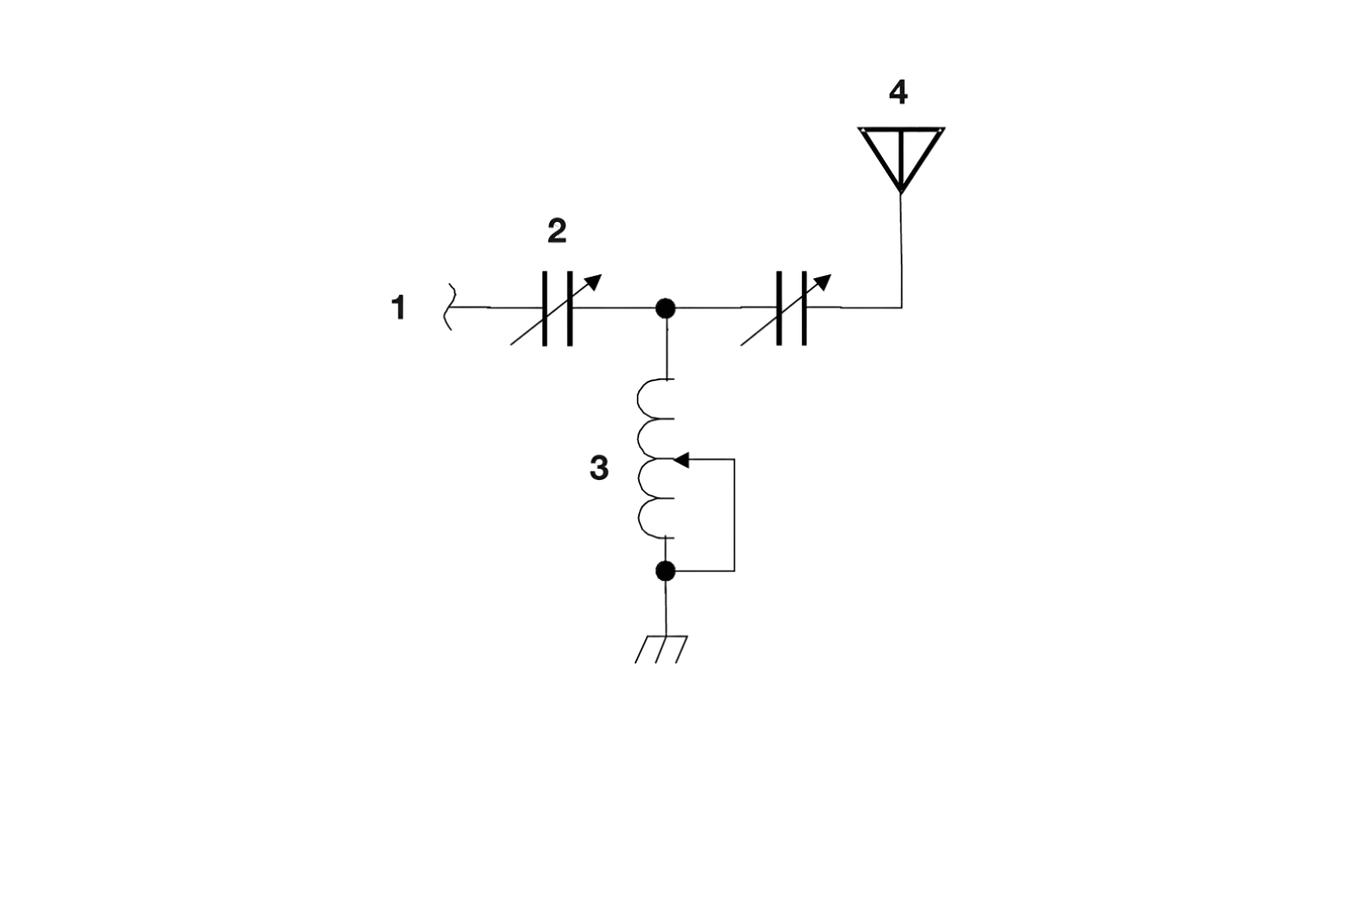
\includegraphics[width=0.7\textwidth]{tech/images/t3.png}
\end{tcolorbox}
Component 4 in figure T-3 is an antenna. Antennas are represented by a line with a small triangle at the end.

\begin{tcolorbox}[colback=gray!10!white,colframe=black!75!black,title={T6C12}]
    Which of the following is accurately represented in electrical schematics?
    \begin{enumerate}[label=\Alph*),noitemsep]
        \item Wire lengths
        \item Physical appearance of components
        \item \textbf{Component connections}
        \item All these choices are correct
    \end{enumerate}
\end{tcolorbox}
Component connections are accurately represented in electrical schematics. Wire lengths and physical appearances are not typically shown in schematics.
